\section{8.26}
\subsection{b)}
\paragraph{Requirements:}
Check if these points form a right angled triangle:
\begin{align*}
    A(-1|-2) &&
    B(1|-3) &&
    C(4|2) \\[20pt]
\end{align*}

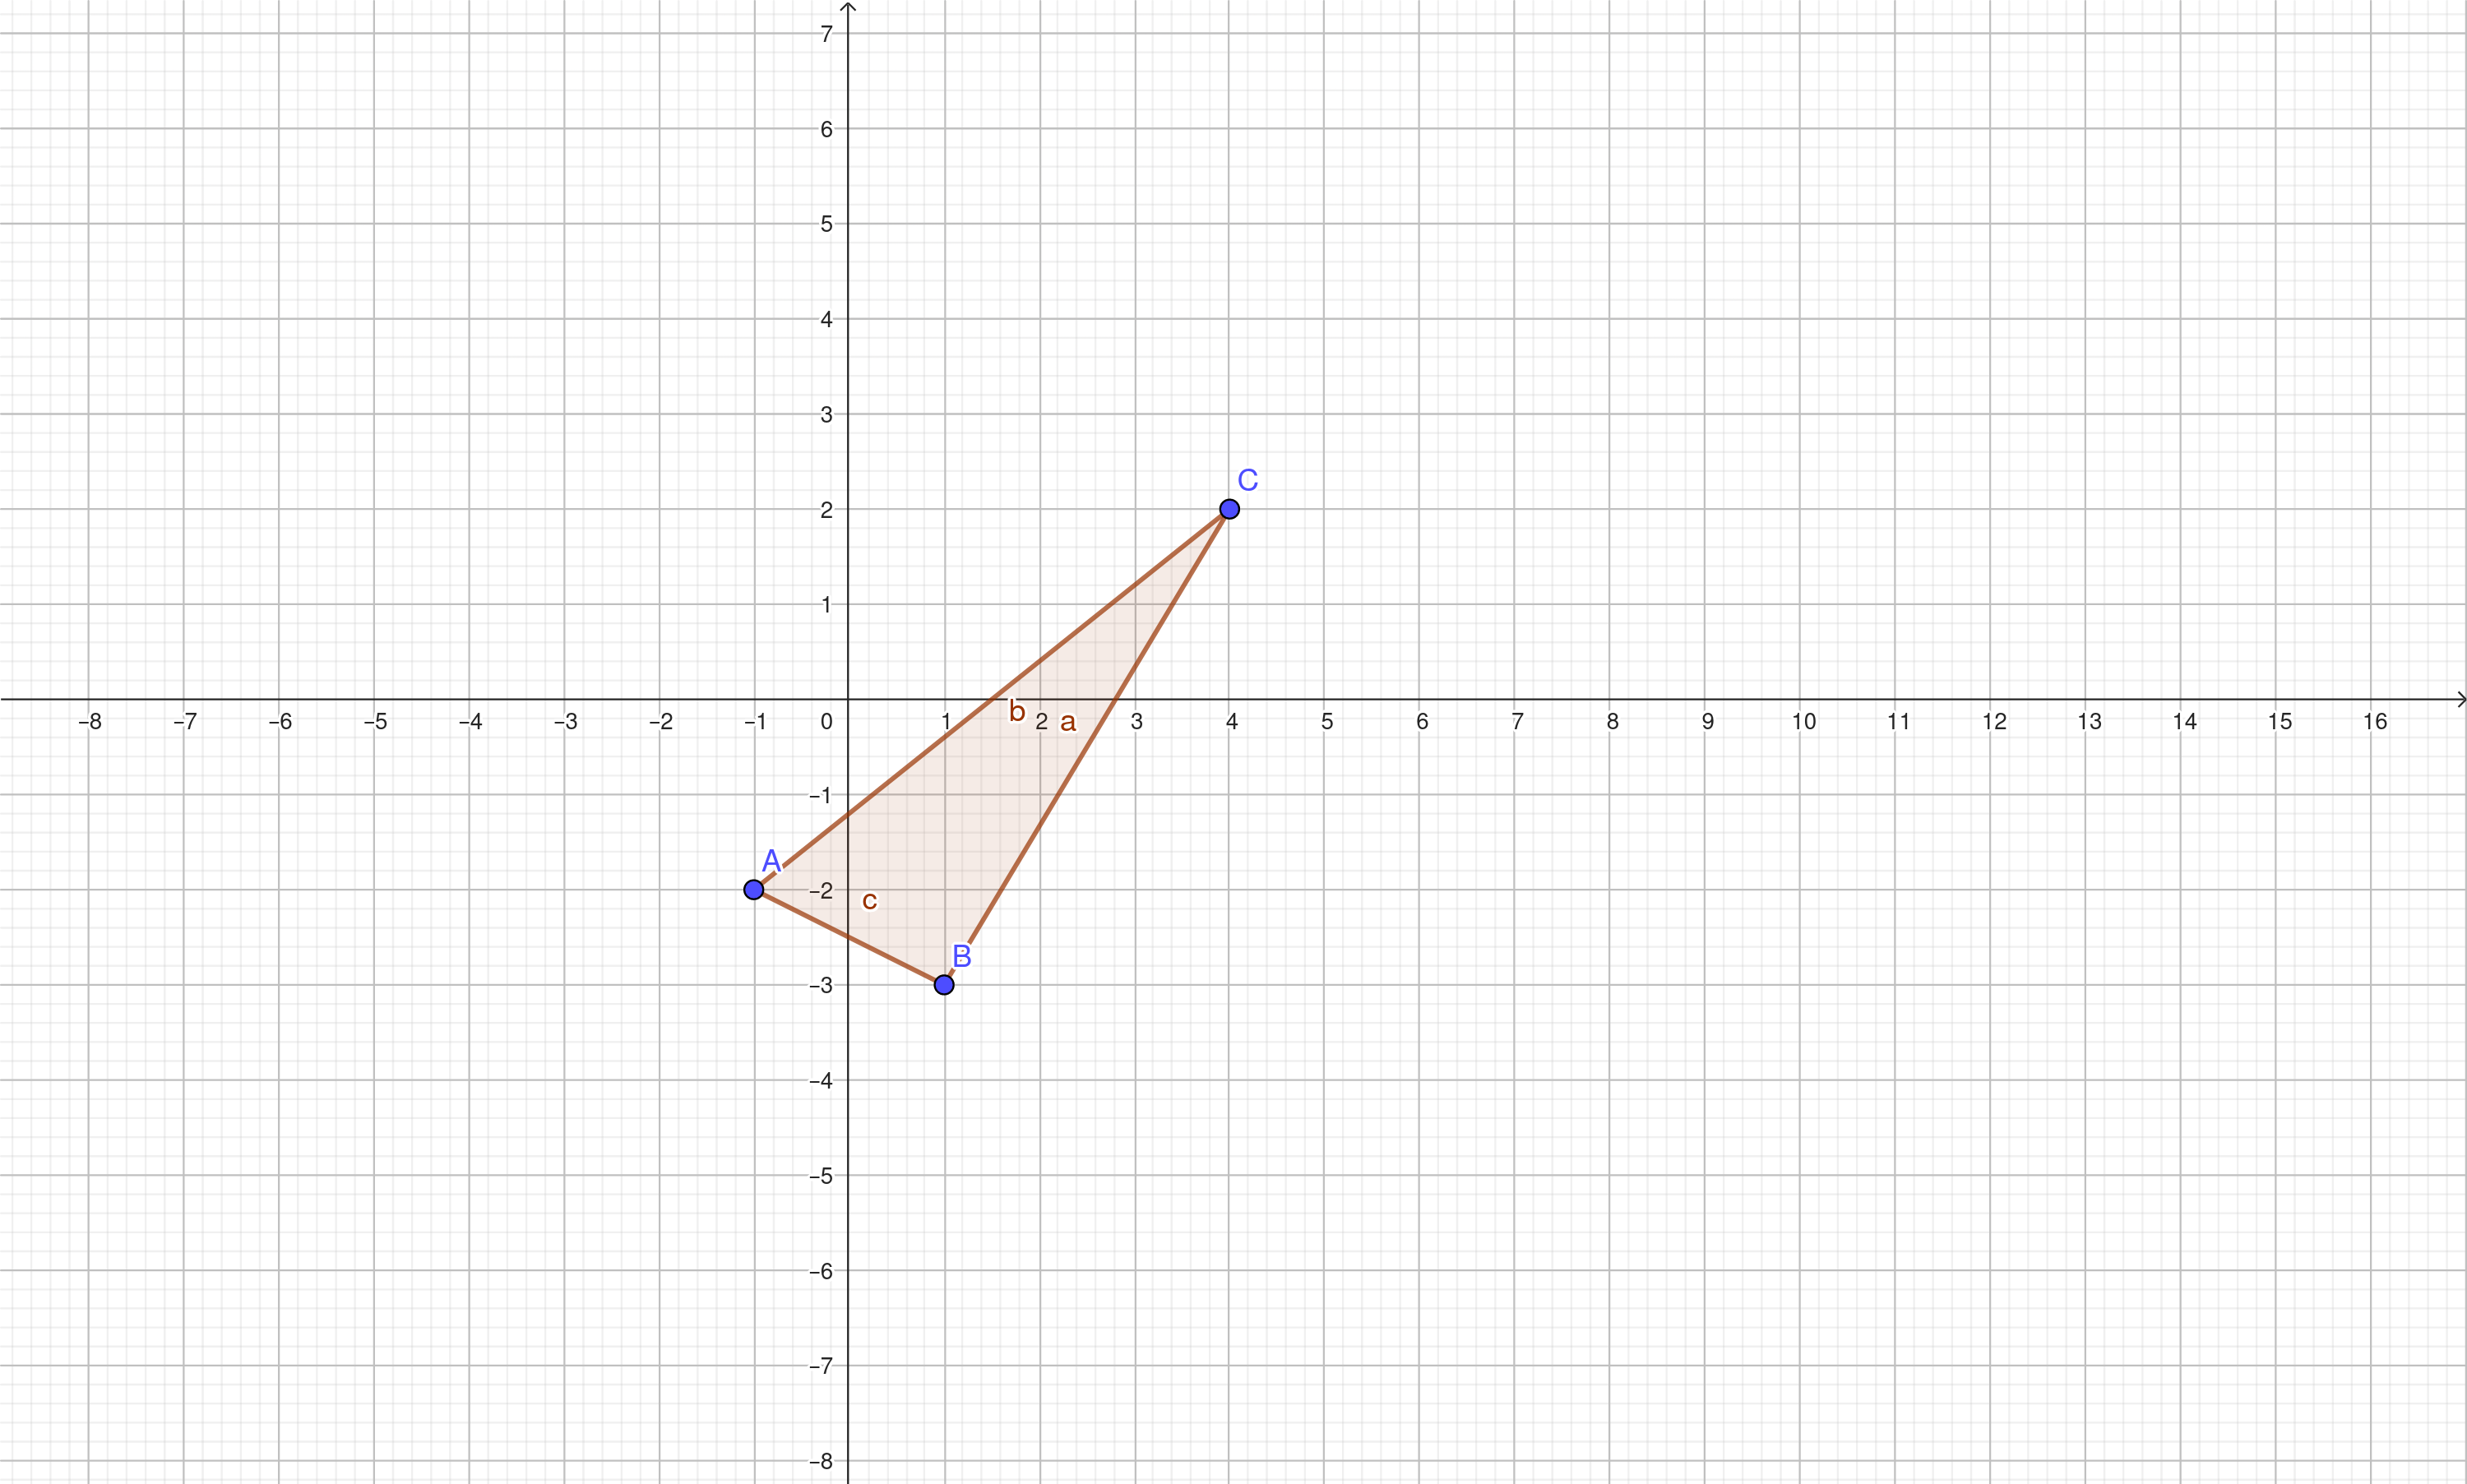
\includegraphics[width=\linewidth]{images/8-26-b.png}

\paragraph{Exercises:}
\begin{align}
    \vec{BC} \cdot \vec{CA} &= BC_x * CA_x + BC_y * CA_y \\
    \vec{BC} \cdot \vec{CA} &= -1 * 1 + -2 * -3 \\
    \vec{BC} \cdot \vec{CA} &= -1 + 6 \\
    \vec{BC} \cdot \vec{CA} &= 5 \\[20pt]
    \vec{BC} \cdot \vec{AB} &= BC_x * AB_x + BC_y * AB_y \\
    \vec{BC} \cdot \vec{AB} &= -1 * 4 + -2 * 2 \\
    \vec{BC} \cdot \vec{AB} &= -4 + -4 \\
    \vec{BC} \cdot \vec{AB} &= -8 \\[20pt]
    \vec{CA} \cdot \vec{AB} &= CA_x * AB_x + CA_y * AB_y \\
    \vec{CA} \cdot \vec{AB} &= 1 * 4 + -3 * 2 \\
    \vec{CA} \cdot \vec{AB} &= 4 + -6 \\
    \vec{CA} \cdot \vec{AB} &= -2
\end{align}

\paragraph{Answer:}
The triangle is not a right angle as none of the angles $\alpha$, $\beta$, $\gamma$ are $90^\circ$.
This is shown be the fact that none of the dot products of the triangles sides are 0.
